\chapter{Badania końcowe i wnioski projektowe}

\section{Cel eksperymentu}
Celem badania było empiryczne porównanie wpływu dwóch podejść do projektowania interfejsu użytkownika oraz wybranych mechanizmów interakcji w wirtualnym środowisku. Analiza obejmowała typ interfejsu, sposób przemieszczania się oraz intensywność informacji zwrotnej, rozumianą jako liczba kanałów komunikujących reakcję systemu na działania użytkownika. Porównanie obu wariantów przeprowadzono w kontrolowanych warunkach, przy zachowaniu identycznej struktury zadań, układu przestrzeni oraz celów do wykonania. Różnice pomiędzy wariantami ograniczono wyłącznie do badanych zmiennych, co umożliwiło zestawienie wyników ilościowych oraz obserwowanych zachowań użytkowników i ocenę wpływu decyzji projektowych na przebieg wykonywania zadań. Jednocześnie zadania zaprojektowano tak, aby przy możliwie ograniczonym zakresie zmian zachować podstawowe interakcje charakterystyczne i wymagane dla analizowanego typu gry.
 
\section{Metodologia badań}

 Zakres badanych obszarów został wyselekcjonowany na podstawie wcześniejszych wyników analizy heurystycznej oraz badania ankietowego. Do badań włączono te aspekty interakcji, które okazały się problematyczne lub niejednoznaczne w obu etapach analizy. Jednym z najczęściej wskazywanych problemów w doświadczeniach VR były mechanizmy lokomocji. Informacja zwrotna, mimo że nie była wskazywana przez użytkowników jako obszar krytyczny, została uwzględniona w badaniu ze względu na wyniki analizy heurystycznej. W większości analizowanych gier VR była ona ograniczona lub pomijana, dlatego zdecydowano się na jej uwzględnienie w badaniu końcowym w celu oceny wpływu intensywności informacji zwrotnej na jakość rozgrywki i przebieg interakcji.
 
 Z zakresu badań świadomie zrezygnowano również z mechaniki ekwipunku, pomimo problemów wykrytych w pierwszym etapie analizy. Decyzja ta wynikała z faktu, że zidentyfikowane trudności dotyczyły wyłącznie jednego typu rozwiązania, tj. ekwipunku realizowanego w formie panelu osadzonego w przestrzeni. Pozostałe warianty uzyskały dobre oceny użyteczności i były wskazywane w badaniu ankietowym jako rozwiązania udane. Uznano zatem, że uwzględnienie mechaniki ekwipunku nie wniesie istotnej wartości do dalszych badań, a zakres pracy zawężono do obszarów generujących największe i najczęściej występujące problemy użytkowe. Dodatkowo obszar ten pokrywał się częściowo funkcjonalnie z interfejsem panelowym, który został już objęty zakresem badania.
W celu wyeliminowania efektu uczenia się badanie zostało zaprojektowane zgodnie z modelem międzygrupowym i przeprowadzone stacjonarnie. Uczestnicy zostali podzieleni na dwie niezależne grupy badawcze, a każda z nich testowała jeden wariant interfejsu. Wybór projektu międzygrupowego został podyktowany obawą, że schemat wewnątrzgrupowy mógłby prowadzić do zapamiętania schematu zadania przez użytkowników i zakłócenia wyników. W badaniu wzięło udział 10 dorosłych osób a rekrutacja odbywała się wśród znajomych i rodziny. Wybrano 6 osób, które miały niewielką styczność ze środowiskiem wirtualnym, nieprzekraczającą około 30 minut wcześniejszego kontaktu, oraz 4 osoby posiadające minimum 10h doświadczenia z urządzeniami VR. Przydzielenie osób doświadczonych i początkujących odbyło się losowo, tak aby powstałe grupy były równo zróżnicowane pod względem poziomu zaawansowania z technologią VR. Decyzja o takim podziale wynikała z wyników ankiet, w których to duża część ankietowanych wskazała na jednokrotne korzystanie z tej technologii. Każda z nich zawierała 3 użytkowników początkujących i 2 zaawansowanych. Zapewniło to kontrolę nad możliwym różnym poziomem doświadczenia osób badanych i pozwoliło na sprawdzenie, czy wcześniejsze doświadczenie wpłynie na odbiór danego wariantu. 

	\begin{figure}[!htb]
  \centering
  \includegraphics[width=1
  \textwidth]{images/chapter6/1.png}
  \caption{Schemat przebiegu eksperymentu międzygrupowego w VR., (2026); Opracowanie: własne}
  \end{figure}


Zaprojektowane zadania nie miały określonego limitu czasu na zadanie aby umożliwić naturalne zachowanie i swobodną eksplorację. W przypadku trudności badanie nie było przerywane, ale dopuszczono przerwy spowodowane złym samopoczuciem. Aby nie wpływać na przebieg badania podczas wykonywania zadań nie udzielano żadnych podpowiedzi. Dane ilościowe były zapisywane automatycznie przez system. Badanie opierało się na metrykach zapisywanych przez system oraz notatkach z sesji obejmujących obserwacje zachowań i krótkie, spontaniczne uwagi uczestników.

Zastosowanie tej metody miało na celu weryfikację, w jakim stopniu dany prototyp wspiera użytkownika w wykonywaniu założonych czynności \cite{Interakcja}. Dodatkową zaletą obserwacji była możliwość identyfikacji przyczyn zróżnicowanych wyników między poszczególnymi scenariuszami, co pozwoliło określić, które elementy środowiska sprzyjają efektywnej interakcji, a które wymagają dalszych modyfikacji i optymalizacji.

\section{Wyniki i obserwacje}

\subsection{Wyniki}

Czas wykonania zadań rejestrowano automatycznie przez system w sekundach, z dokładnością do dwóch miejsc po przecinku. Jest to podstawowa metryka użyteczności, opisująca czas potrzebny użytkownikowi do ukończenia zdefiniowanego zadania \cite{Pomiary}. Po badaniu dane eksportowano do pliku \texttt{.txt}, natomiast obserwacje jakościowe zapisywano odręcznie na tablecie w trakcie trwania eksperymentu. W tabelach zestawiono czasy wykonania zadań oraz liczbę niepowodzeń. Jako niepowodzenie (N) w zadaniu 1 uznawano upuszczenie przenoszonego przedmiotu. W zadaniu 2 niepowodzenie stanowiło wprowadzenie błędnej sekwencji. W zadaniach 3 i 4 za niepowodzenie przyjmowano upadek użytkownika (np. spadnięcie z przeszkody lub platformy), skutkujący koniecznością cofnięcia się i ponownej próby.

\subsubsection{Zależności w scenariuszu A}


\begin{table}[htbp]
\centering
\caption{Wyniki wykonania zadań w scenariuszu A (czas oraz liczba niepowodzeń $N$)}
\label{tab:scenariuszA_wyniki}
\renewcommand{\arraystretch}{1.2}
\setlength{\tabcolsep}{3pt}
\footnotesize

\resizebox{\textwidth}{!}{%
\begin{tabular}{|c|c|c|c|c|c|c|c|c|c|c|}
\hline
\textbf{Użytkownik} & \textbf{Poziom} &
\multicolumn{2}{c|}{\textbf{Zadanie 1}} &
\multicolumn{2}{c|}{\textbf{Zadanie 2}} &
\multicolumn{2}{c|}{\textbf{Zadanie 3}} &
\multicolumn{2}{c|}{\textbf{Zadanie 4}} &
\textbf{Czas ukończenia} \\
\cline{3-10}
 & &
\textbf{Czas [s]} & \textbf{$N$} &
\textbf{Czas [s]} & \textbf{$N$} &
\textbf{Czas [s]} & \textbf{$N$} &
\textbf{Czas [s]} & \textbf{$N$} &
\textbf{scenariusza [s]} \\
\hline
U1 & Początkujący & 104,54 & 0 & 98,16 & 2 & 84,75 & 1 & 78,52 & 0 & 365,97 \\
U2 & Początkujący & 96,85 & 0 & 93,23 & 2 & 118,09 & 4 & 106,98 & 1 & 415,15 \\
U3 & Początkujący & 110,98 & 1 & 123,02 & 4 & 99,11 & 2 & 69,75 & 0 & 402,86 \\
U4 & Zaawansowany & 78,31 & 0 & 78,32 & 0 & 27,98 & 0 & 55,43 & 0 & 240,04 \\
U5 & Zaawansowany & 73,73 & 0 & 65,25 & 0 & 37,77 & 0 & 59,01 & 0 & 235,76 \\
\hline
\multicolumn{2}{|l|}{\textbf{Średnia czasu / osoby z niepowodzeniem (Początkujący)}} &
104,12 & 1/3 & 104,80 & 3/3 & 100,65 & 3/3 & 85,08 & 1/3 & 394,66 \\
\hline
\multicolumn{2}{|l|}{\textbf{Średnia czasu / osoby z niepowodzeniem (Zaawansowani)}} &
76,02 & 0/2 & 71,79 & 0/2 & 32,88 & 0/2 & 57,22 & 0/2 & 237,90 \\
\hline
\end{tabular}%
}

\vspace{0.5em}
\footnotesize
\textbf{Uwaga:} $N$ oznacza liczbę niepowodzeń w zadaniu. W wierszach podsumowania podano średni czas oraz liczbę osób z co najmniej jednym niepowodzeniem w formacie $k/n$.
\end{table}




W scenariuszu A czas ukończenia scenariusza jest sumą czasów czterech zadań dla danego uczestnika (kolumny "Czas na zadanie" dla zadań 1-4 sumują się do kolumny "Czas ukończenia scenariusza") (tab. \ref{tab:scenariuszA_wyniki}). Oznacza to, że wydłużenie dowolnego zadania bezpośrednio przekłada się na wynik końcowy.

W perspektywie grupowej uczestnicy zaawansowani osiągnęli niższe czasy w każdym zadaniu oraz niższy czas ukończenia scenariusza (średnio 237,90~s) niż początkujący (394,66~s) (tab. \ref{tab:scenariuszA_wyniki}). W grupie zaawansowanej nie wystąpiły niepowodzenia w żadnym zadaniu (0/2 we wszystkich kolumnach $N$), natomiast w grupie początkującej niepowodzenia koncentrowały się w zadaniach 2 i 3 (odpowiednio 3/3 osób z niepowodzeniem).

Wśród początkujących zadanie 2 i zadanie 3 charakteryzowały się jednocześnie wysokim odsetkiem niepowodzeń oraz relatywnie wysokimi czasami (średnio 104,80~s oraz 100,65~s). W danych jednostkowych widać współwystępowanie większej liczby niepowodzeń z dłuższym czasem realizacji w zadaniu 2 (np. U3: $N=4$, 123,02~s) oraz w zadaniu 3 (np. U2: $N=4$, 118,09~s) (tab. \ref{tab:scenariuszA_wyniki}). Zmienność czasu ukończenia scenariusza była większa wśród początkujących (365,97-415,15~s) niż wśród zaawansowanych (235,76-240,04~s).




\subsubsection{Zależności w scenariuszu B}

\begin{table}[htbp]
\centering
\caption{Wyniki wykonania zadań w scenariuszu B (czas oraz liczba niepowodzeń $N$)}
\label{tab:scenariuszB_wyniki}
\renewcommand{\arraystretch}{1.2}
\setlength{\tabcolsep}{3pt}
\footnotesize

\resizebox{\textwidth}{!}{%
\begin{tabular}{|c|c|c|c|c|c|c|c|c|c|c|}
\hline
\textbf{Użytkownik} & \textbf{Poziom} &
\multicolumn{2}{c|}{\textbf{Zadanie 1}} &
\multicolumn{2}{c|}{\textbf{Zadanie 2}} &
\multicolumn{2}{c|}{\textbf{Zadanie 3}} &
\multicolumn{2}{c|}{\textbf{Zadanie 4}} &
\textbf{Czas ukończenia} \\
\cline{3-10}
 & &
\textbf{Czas [s]} & \textbf{$N$} &
\textbf{Czas [s]} & \textbf{$N$} &
\textbf{Czas [s]} & \textbf{$N$} &
\textbf{Czas [s]} & \textbf{$N$} &
\textbf{scenariusza [s]} \\
\hline
U6 & Początkujący & 148,26 & 1 & 88,99 & 1 & 74,55 & 1 & 139,97 & 1 & 451,77 \\
U7 & Początkujący & 124,65 & 0 & 79,95 & 1 & 67,91 & 0 & 220,28 & 3 & 492,79 \\
U8 & Początkujący & 131,93 & 1 & 82,91 & 1 & 68,37 & 0 & 90,91 & 0 & 374,12 \\
U9 & Zaawansowany & 87,17 & 0 & 52,02 & 0 & 20,93 & 0 & 54,21 & 0 & 214,33 \\
U10 & Zaawansowany & 82,58 & 0 & 51,25 & 0 & 22,62 & 0 & 56,66 & 0 & 213,11 \\
\hline
\multicolumn{2}{|l|}{\textbf{Średnia czasu / osoby z niepowodzeniem (Początkujący)}} &
134,95 & 2/3 & 83,95 & 3/3 & 70,28 & 1/3 & 150,39 & 2/3 & 439,56 \\
\hline
\multicolumn{2}{|l|}{\textbf{Średnia czasu / osoby z niepowodzeniem (Zaawansowani)}} &
84,88 & 0/2 & 51,64 & 0/2 & 21,78 & 0/2 & 55,44 & 0/2 & 213,72 \\
\hline
\end{tabular}%
}

\vspace{0.5em}
\footnotesize
\textbf{Uwaga:} $N$ oznacza liczbę niepowodzeń w zadaniu. W wierszach podsumowania podano średni czas oraz liczbę osób z co najmniej jednym niepowodzeniem w formacie $k/n$.
\end{table}


Analogicznie do scenariusza A, w scenariuszu B czas ukończenia scenariusza stanowi sumę czasów czterech zadań dla danego uczestnika (tab. \ref{tab:scenariuszB_wyniki}). Z punktu widzenia analizy oznacza to, że zadania o największych czasach mają największy wkład w wynik końcowy.

Uczestnicy zaawansowani uzyskali niższe czasy w każdym zadaniu oraz niższy czas ukończenia scenariusza (średnio 213,72~s) niż początkujący (439,56~s) (tab. \ref{tab:scenariuszB_wyniki}). W grupie zaawansowanej nie odnotowano niepowodzeń (0/2 w każdej kolumnie $N$), natomiast w grupie początkującej niepowodzenia wystąpiły we wszystkich zadaniach, przy czym najczęściej w zadaniu 2 (3/3) oraz w zadaniu 1 i 4 (po 2/3).

Wśród początkujących zadanie 4 wykazuje największą średnią wartość czasu (150,39~s) oraz jednocześnie podwyższoną liczbę niepowodzeń (2/3 osób z niepowodzeniem). W danych jednostkowych widoczny jest wynik odstający w zadaniu 4 (U7: 220,28~s i $N=3$), który zwiększa rozpiętość czasu ukończenia scenariusza w tej grupie (374,12-492,79~s) (tab. \ref{tab:scenariuszB_wyniki}). Dla zaawansowanych rozpiętość czasu ukończenia scenariusza jest minimalna (213,11-214,33~s).


\subsection{Porównanie wyników ilościowych między wariantami}

\subsubsection{Porównanie median czasów zadań między wariantami}



\begin{figure}[htbp]
\centering
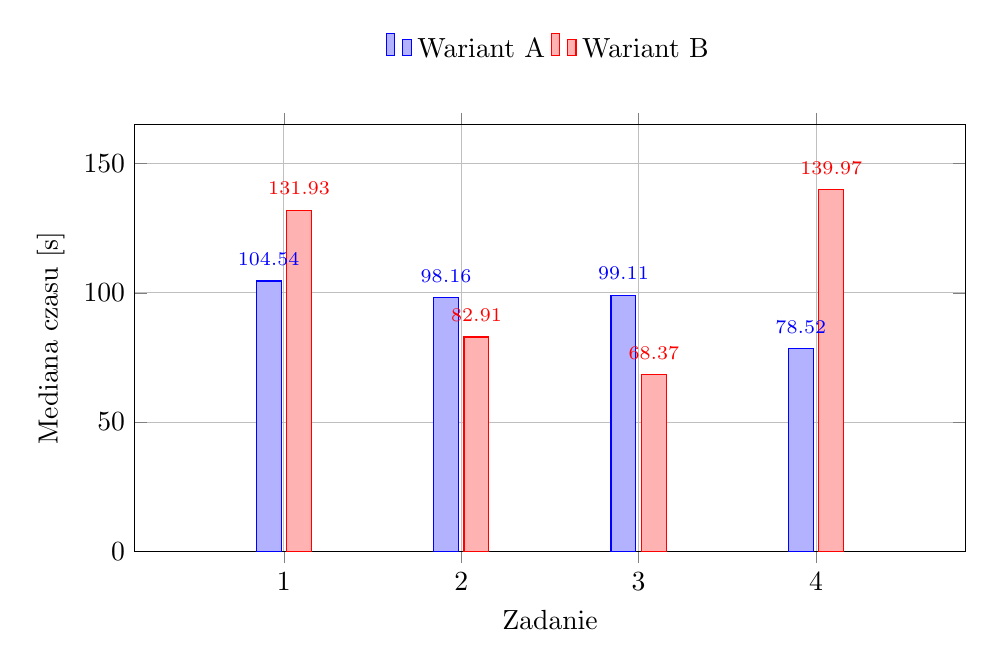
\begin{tikzpicture}
\begin{axis}[
    ybar,
    width=\textwidth,
    height=7cm,
    bar width=9pt,
    ymin=0,
    ymax=165,
    ylabel={Mediana czasu [s]},
    xlabel={Zadanie},
    symbolic x coords={1,2,3,4},
    xtick=data,
    enlarge x limits=0.28,
    grid=both,
    legend style={
        at={(0.5,1.12)},
        anchor=south,
        draw=none,
        fill=none,
        legend columns=2
    },
    nodes near coords,
    every node near coord/.append style={font=\scriptsize, yshift=2pt},
]

\addplot coordinates {(1,104.54) (2,98.16) (3,99.11) (4,78.52)};
\addlegendentry{Wariant A}

\addplot coordinates {(1,131.93) (2,82.91) (3,68.37) (4,139.97)};
\addlegendentry{Wariant B}

\end{axis}
\end{tikzpicture}
\caption{Porównanie median czasu wykonania zadań 1-4 (początkujący): wariant A vs wariant B.}
\label{fig:slupki_mediany_pocz_A_B}
\end{figure}

\noindent\textbf{Początkujący}
Porównanie median czasów wykonania zadań wskazuje, że w wariancie B mediana była wyższa niż w wariancie A w zadaniu 1 (131,93~s vs 104,54~s) oraz w zadaniu 4 (139,97~s vs 78,52~s), natomiast niższa w zadaniu 2 (82,91~s vs 98,16~s) i w zadaniu 3 (68,37~s vs 99,11~s) (rys. \ref{fig:slupki_mediany_pocz_A_B}). Największa różnica median dotyczy zadania 4, gdzie wariant B osiągnął wynik wyższy o 61,45~s.


\begin{figure}[htbp]
\centering
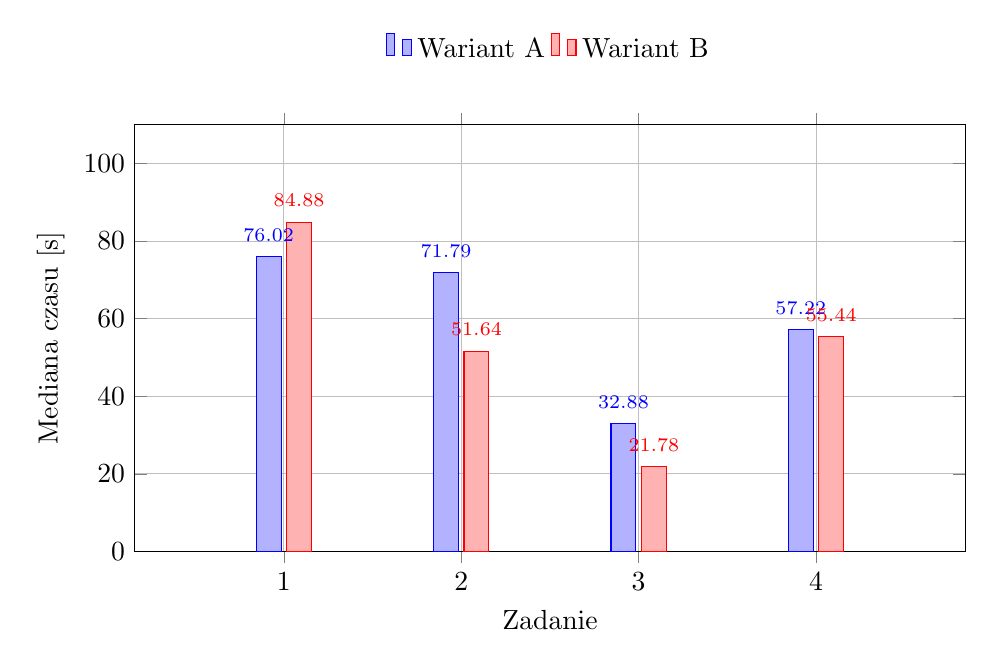
\begin{tikzpicture}
\begin{axis}[
    ybar,
    width=\textwidth,
    height=7cm,
    bar width=9pt,
    ymin=0,
    ymax=110,
    ylabel={Mediana czasu [s]},
    xlabel={Zadanie},
    symbolic x coords={1,2,3,4},
    xtick=data,
    enlarge x limits=0.28,
    grid=both,
    legend style={
        at={(0.5,1.12)},
        anchor=south,
        draw=none,
        fill=none,
        legend columns=2
    },
    nodes near coords,
    every node near coord/.append style={font=\scriptsize, yshift=2pt},
]

% Wariant A — zaawansowani (mediany)
\addplot coordinates {(1,76.02) (2,71.785) (3,32.875) (4,57.22)};
\addlegendentry{Wariant A}

% Wariant B — zaawansowani (mediany)
\addplot coordinates {(1,84.875) (2,51.635) (3,21.775) (4,55.435)};
\addlegendentry{Wariant B}

\end{axis}
\end{tikzpicture}
\caption{Porównanie median czasu wykonania zadań 1-4 (zaawansowani): wariant A vs wariant B.}
\label{fig:slupki_mediany_zaaw_A_B}
\end{figure}

\FloatBarrier

\noindent\textbf{Zaawansowani}
W grupie zaawansowanej wariant B osiągnął wyższą medianę czasu w zadaniu 1 (84,875~s vs 76,02~s), natomiast niższe mediany w zadaniu 2 (51,635~s vs 71,785~s), zadaniu 3 (21,775~s vs 32,875~s) oraz zadaniu 4 (55,435~s vs 57,22~s) (rys. \ref{fig:slupki_mediany_zaaw_A_B}). Największa różnica median wystąpiła w zadaniu 2 (spadek o 20,15~s w wariancie B).


\subsubsection{Podsumowanie wyników ilościowych}

W ujęciu scenariusza jako całości, w grupie początkującej wariant B miał wyższy średni czas ukończenia scenariusza niż wariant A (439,56~s vs 394,66~s), a jednocześnie niższą średnią liczbę niepowodzeń na osobę (3,33 vs 5,67) (tab. \ref{tab:podsumowanie_ilosciowe}). W grupie zaawansowanej wariant B osiągnął niższy średni czas ukończenia scenariusza niż wariant A (213,72~s vs 237,90~s), przy braku niepowodzeń w obu wariantach (0,00 $N$/os.) (tab. \ref{tab:podsumowanie_ilosciowe}).

\begin{table}[htbp]
\centering
\caption{Podsumowanie wyników ilościowych (czas scenariusza i liczba niepowodzeń $N$)}
\label{tab:podsumowanie_ilosciowe}
\renewcommand{\arraystretch}{1.2}
\setlength{\tabcolsep}{6pt}
\footnotesize
\begin{tabular}{|c|c|c|c|c|}
\hline
\textbf{Wariant} & \textbf{Grupa} & \textbf{$n$} & \textbf{Śr. czas scenariusza [s]} & \textbf{Śr. $N$/os. (suma $N$)} \\
\hline
A & Początkujący & 3 & 394,66 & 5,67  (17) \\
A & Zaawansowani  & 2 & 237,90 & 0,00  (0) \\
\hline
B & Początkujący & 3 & 439,56 & 3,33  (10) \\
B & Zaawansowani  & 2 & 213,72 & 0,00  (0) \\
\hline
\end{tabular}
\end{table}




W obu wariantach odnotowano silny wpływ doświadczenia na efektywność realizacji zadań. W scenariuszu A grupa początkująca ukończyła scenariusz średnio w 394,66 s, natomiast grupa zaawansowana w 237,90 s (tab. \ref{tab:scenariuszA_wyniki}).W wariancie B (scenariusz B) średni czas ukończenia wyniósł odpowiednio 439,56~s dla początkujących oraz 213,72~s dla zaawansowanych (tab. \ref{tab:scenariuszB_wyniki}). W obu scenariuszach użytkownicy zaawansowani nie odnotowali niepowodzeń (0/2), co wskazuje na stabilne wykonywanie interakcji niezależnie od wariantu.
% -- Interfejs i wskazówki --
\begin{table}[htbp]
\centering
\caption{Obserwacje jakościowe: Interfejs i wskazówki}
\label{tab:obs_interfejs_wskazowki}
\renewcommand{\arraystretch}{1.2}
\setlength{\tabcolsep}{4pt}
\footnotesize
\resizebox{\textwidth}{!}{%
\begin{tabular}{|l|c|c|l|p{0.55\textwidth}|}
\hline
\textbf{Uczestnik} & \textbf{Wariant} & \textbf{Zadanie} & \textbf{Etap} & \textbf{Obserwacja} \\
\hline
U2  & A & 1 & początkowy & Uczestnik po wejściu do przestrzeni zadania od razu skierował uwagę na panel i skorzystał z niego jako pierwszego źródła informacji. \\
\hline
U6  & B & 1 & początkowy & Uczestnik rozpoczął wykonywanie czynności w zadaniu bez wcześniejszego spojrzenia na nadgarstek; dopiero po pewnym czasie skierował wzrok na zegarek. \\
\hline
U7  & B & 2 & po pierwszej nieudanej interakcji & Uczestnik wielokrotnie spoglądał na nadgarstek w trakcie wykonywania zadania (powtarzalne korzystanie z diegetycznego źródła informacji). \\
\hline
U9  & B & 1 & początkowy & Uczestnik szybko zidentyfikował elementy diegetyczne jako źródło informacji i korzystał z nich w trakcie wykonywania zadania. \\
\hline
U10 & B & 1 & początkowy & Uczestnik szybko zidentyfikował elementy diegetyczne jako źródło informacji i korzystał z nich w trakcie wykonywania zadania. \\
\hline
\end{tabular}%
}
\end{table}

% -- Manipulacja + lokomocja --
\begin{table}[htbp]
\centering
\caption{Obserwacje jakościowe: Manipulacja + lokomocja}
\label{tab:obs_manip_lokomocja}
\renewcommand{\arraystretch}{1.2}
\setlength{\tabcolsep}{4pt}
\footnotesize
\resizebox{\textwidth}{!}{%
\begin{tabular}{|l|c|c|l|p{0.55\textwidth}|}
\hline
\textbf{Uczestnik} & \textbf{Wariant} & \textbf{Zadanie} & \textbf{Etap} & \textbf{Obserwacja} \\
\hline
U3 & A & 1 & początkowy & Uczestnik upuścił przenoszony obiekt w trakcie wykonywania lokomocji/teleportacji (zdarzenie czasowo powiązane z aktywacją przemieszczania). \\
\hline
U6, U8 & B & 1 & początkowy & Uczestnicy upuścił przenoszony obiekt w trakcie wykonywania lokomocji/teleportacji (zdarzenie czasowo powiązane z aktywacją przemieszczania). \\
\hline
\end{tabular}%
}
\end{table}

% -- Informacja zwrotna – przeciążenie bodźcami --
\begin{table}[htbp]
\centering
\caption{Obserwacje jakościowe: Informacja zwrotna - przeciążenie bodźcami}
\label{tab:obs_feedback_bodzce}
\renewcommand{\arraystretch}{1.2}
\setlength{\tabcolsep}{4pt}
\footnotesize
\resizebox{\textwidth}{!}{%
\begin{tabular}{|l|c|c|l|p{0.55\textwidth}|}
\hline
\textbf{Uczestnik} & \textbf{Wariant} & \textbf{Zadanie} & \textbf{Etap} & \textbf{Obserwacja} \\
\hline
U6 & B & 2 & początkowy & Uczestnik zgłosił, że bodźce dźwiękowe są zbyt intensywne i rozpraszają w trakcie zadania wymagającego koncentracji. \\
\hline
U7 & B & 2 & po pierwszej nieudanej próbie & Po sygnale błędu uczestnik odszedł od miejsca wprowadzania sekwencji i rozpoczął eksplorację przestrzeni w poszukiwaniu wskazówek, a następnie wrócił do kolejnej próby. \\
\hline
U3 & A & 2 & po drugiej nieudanej próbie & Po sygnale błędu uczestnik podejmował kolejne próby wprowadzania sekwencji bez natychmiastowej zmiany zachowania (brak odejścia od miejsca wejściowego). \\
\hline
U2 & A & 2 & po drugiej nieudanej próbie & Dopiero po kolejnych sygnałach błędu uczestnik przerwał wpisywanie sekwencji i rozpoczął eksplorację przestrzeni w poszukiwaniu wskazówek. \\
\hline
\end{tabular}%
}
\end{table}

% -- Strategia po błędzie i eksploracja --
\begin{table}[htbp]
\centering
\caption{Obserwacje jakościowe: Strategia po błędzie i eksploracja}
\label{tab:obs_strategia_eksploracja}
\renewcommand{\arraystretch}{1.2}
\setlength{\tabcolsep}{4pt}
\footnotesize
\resizebox{\textwidth}{!}{%
\begin{tabular}{|l|c|c|l|p{0.55\textwidth}|}
\hline
\textbf{Uczestnik} & \textbf{Wariant} & \textbf{Zadanie} & \textbf{Etap} & \textbf{Obserwacja} \\
\hline
U1-U3 & A & 2 & początkowy & Uczestnik po wejściu do przestrzeni zadania przeszedł bezpośrednio do miejsca wprowadzania sekwencji i podjął próbę wykonania zadania bez wcześniejszego wejścia do pomieszczenia z odpowiedziami. \\
\hline
U6-U8 & B & 2 & początkowy & Uczestnik po wejściu do przestrzeni zadania przeszedł bezpośrednio do miejsca wprowadzania sekwencji i podjął próbę wykonania zadania bez wcześniejszego wejścia do pomieszczenia z odpowiedziami. \\
\hline
U1-U2 & A & 2 & po drugiej nieudanej próbie & Uczestnik przerwał kolejne wpisywanie sekwencji, rozpoczął eksplorację przestrzeni i wszedł do pomieszczenia z odpowiedziami. \\
\hline
U6-U8 & B & 2 & po pierwszej nieudanej próbie & Uczestnik odszedł od miejsca wprowadzania sekwencji i rozpoczął eksplorację przestrzeni w kierunku pomieszczenia z odpowiedziami. \\
\hline
U3 & A & 2 & po trzeciej nieudanej próbie & Uczestnik wykonał trzy nieudane próby wprowadzenia sekwencji, a poprawną sekwencję wprowadził w kolejnej próbie przypadkowo. \\
\hline
U1-U2 & A & 2 & po eksploracji & Po zmianie zachowania (odejście i eksploracja) uczestnik wrócił do miejsca wprowadzania sekwencji i wykonał kolejną próbę. \\
\hline
U6-U8 & B & 2 & po eksploracji & Po zmianie zachowania (odejście i eksploracja) uczestnik wrócił do miejsca wprowadzania sekwencji i wykonał kolejną próbę. \\
\hline
\end{tabular}%
}
\end{table}

% -- Lokomocja – dyskomfort i zmiana stylu ruchu --
\begin{table}[htbp]
\centering
\caption{Obserwacje jakościowe: Lokomocja - dyskomfort i zmiana stylu ruchu}
\label{tab:obs_lokomocja_dyskomfort}
\renewcommand{\arraystretch}{1.2}
\setlength{\tabcolsep}{4pt}
\footnotesize
\resizebox{\textwidth}{!}{%
\begin{tabular}{|l|c|c|l|p{0.55\textwidth}|}
\hline
\textbf{Uczestnik} & \textbf{Wariant} & \textbf{Zadanie} & \textbf{Etap} & \textbf{Obserwacja} \\
\hline
U2-U3 & A & 3 & początkowy & Uczestnik zgłosił dyskomfort podczas lokomocji ciągłej (np. mdłości) / przerwał sesję. \\
\hline
U2 & A & 3 & końcowy & Uczestnik poruszał się bardziej oszczędnie niż na początku (częstsze zatrzymania, krótsze przemieszczenia). \\
\hline
U1, U3 & A & 3 & początkowy & Uczestnik spadł z platformy podczas poruszania się lokomocją ciągłą (smooth), co wymusiło powtórzenie fragmentu zadania. \\
\hline
U3 & A & 3 & końcowy & Uczestnik spadł z platformy podczas poruszania się lokomocją ciągłą (smooth), co wymusiło powtórzenie fragmentu zadania. \\
\hline
U7 & B & 4 & końcowy & Uczestnik wykonywał ruchy ciałem/kontrolerami, sugerujące próbę fizycznego „odpychania się” od drążków zamiast aktywacji teleportacji. \\
\hline
U7 & B & 4 & końcowy przemieszczania się fizycznego & Uczestnik poświęcił dłuższy czas na ustawianie celu teleportacji (wskazywanie różnych punktów) przed skutecznym przemieszczeniem. \\
\hline
U6 & B & 4 & końcowy & Uczestnik podczas próby teleportacji zwolnił przycisk odpowiedzialny za utrzymanie chwytu drążka, co doprowadziło do utraty podparcia i niepowodzenia. \\
\hline
\end{tabular}%
}
\end{table}


\section{Interpretacja wyników i wnioski projektowe}

\subsection{Interpretacja wyników}

Analiza zgromadzonych danych ilościowych oraz obserwacji jakościowych pozwoliła na weryfikację założeń projektowych sformułowanych na etapie analizy gier i badania ankietowego. Wyniki eksperymentu potwierdziły, że wybór podejścia do projektowania interfejsu i interakcji ma kluczowe znaczenie dla komfortu i efektywności użytkownika, a różnice te są szczególnie widoczne przy uwzględnieniu poziomu doświadczenia badanych.

W zadaniu 1 użytkownicy początkujący osiągnęli lepszą efektywność w wariancie A niż w wariancie B, co przejawiało się krótszym czasem realizacji oraz mniejszą liczbą sytuacji przerywających przebieg zadania. Jednym z czynników różnicujących było tempo rozpoczęcia działania: w wariancie A panel był zauważalny natychmiast po wejściu do przestrzeni zadania, co sprzyjało szybkiemu przejściu do właściwej realizacji celu. W wariancie B odnotowano przypadek, w którym uczestnik rozpoczął wykonywanie zadania bez wcześniejszego skorzystania z diegetycznego źródła informacji (np. zegarka) oraz bez odniesienia do wskazówek umieszczonych w środowisku, co mogło wydłużyć czas wstępnej orientacji.

Różnice pomiędzy grupą początkującą i zaawansowaną były widoczne w obu wariantach. U uczestników mniej doświadczonych częściej obserwowano zachowania eksploracyjne przed podjęciem decyzji o kolejnych działaniach, co mogło przekładać się na dłuższy czas realizacji. Ponadto część niepowodzeń w grupie początkującej była powiązana czasowo z koniecznością jednoczesnego utrzymywania obiektu i wykonywania działań lokomocyjnych, co zwiększało obciążenie sterowania i prowadziło do upuszczeń. W grupie zaawansowanej diegetyczny interfejs oraz wskazówki środowiskowe były natomiast rozpoznawane szybciej: uczestnicy wcześniej wykazywali świadomość istnienia tych elementów i korzystali z nich w trakcie wykonywania zadania, co ograniczało koszt „odkrywania” informacji i stabilizowało przebieg interakcji.

W zadaniu 2 zarówno użytkownicy początkujący, jak i zaawansowani uzyskali gorsze wyniki w porównaniu z pozostałymi zadaniami, co wskazuje na wyższy poziom złożoności tego etapu. W grupie zaawansowanej różnice pomiędzy wariantami były niewielkie, natomiast większe zróżnicowanie zaobserwowano w grupie początkującej. Obserwacje z sesji sugerują, że istotnym czynnikiem wpływającym na liczbę niepowodzeń była początkowa strategia działania i sposób eksploracji przestrzeni. W wariancie A część uczestników przechodziła bezpośrednio do miejsca wprowadzania sekwencji, podejmując kolejne próby bez wcześniejszego odnalezienia źródła poprawnej odpowiedzi w środowisku („pokój z odpowiedziami”). Dopiero po kolejnych nieudanych próbach u części osób następowała zmiana zachowania polegająca na rozpoczęciu eksploracji pomieszczenia w celu znalezienia wskazówek, natomiast w pojedynczym przypadku poprawna sekwencja została wprowadzona po kilku próbach bez wyraźnej zmiany strategii. W wariancie B odnotowano natomiast, że u użytkowników początkujących już po pierwszej nieudanej próbie następowała zmiana zachowania polegająca na odejściu od miejsca wprowadzania sekwencji i rozpoczęciu przeszukiwania przestrzeni, co mogło ograniczać liczbę kolejnych błędów w tym zadaniu.

W obu wariantach w zadaniach 3 i 4 zaobserwowano, że osoby doświadczone szybko adaptowały się do zastosowanego mechanizmu lokomocji, niezależnie od tego, czy był to ruch płynny, czy teleportacja. Jednocześnie część uczestników z grupy zaawansowanej spontanicznie deklarowała preferencję dla swobodnego przemieszczania się, a teleportacja była komentowana jako rozwiązanie mniej satysfakcjonujące w odbiorze, mimo że w wariancie z teleportacją osiągano krótsze czasy realizacji. W grupie początkującej w scenariuszu z lokomocją ciągłą odnotowano natomiast większe trudności w przechodzeniu fragmentów planszy, obejmujące zgłaszany dyskomfort oraz większą liczbę upadków z platform, co przekładało się na wydłużenie czasu i konieczność ponawiania prób. W scenariuszu z teleportacją wyniki początkujących były bardziej zbliżone do wyników osób zaawansowanych, co sugeruje, że w tej konfiguracji badania teleportacja ograniczała koszt opanowania przemieszczania się u mniej doświadczonych uczestników, zwłaszcza w zadaniach wymagających precyzyjnego ustawiania pozycji na platformach.

W zadaniu 4 zaobserwowano wyraźne zróżnicowanie czasów wykonania w obrębie tej samej grupy, w tym pojedynczy wynik odstający, który istotnie zawyżał zróżnicowanie. Z obserwacji przebiegu sesji wynika, że w przypadku jednej osoby wydłużenie czasu było powiązane z próbami wykonania przemieszczenia metodą ruchu fizycznego w miejscu, w którym w wariancie przewidziano użycie teleportacji. Uczestnik podejmował kilkukrotne próby „rozbujania się” na drążkach w celu doskoku do kolejnego fragmentu, a kolejne podejścia kończyły się niepowodzeniem i wymuszały ponowienie etapu. W tym samym zadaniu odnotowano również niepowodzenia związane z upadkami: w jednym przypadku do upadku doszło podczas przemieszczania się z wykorzystaniem ruchu fizycznego, a w innym podczas przechodzenia z drążków zawieszonych w przestrzeni na platformę.

W tym samym wariancie pojawił się przypadek pojedynczego błędu, którego przebieg był odmienny: uczestnik podejmował próbę teleportacji, jednak w trakcie tej czynności zwolnił przycisk odpowiedzialny za utrzymanie chwytu drążka, co doprowadziło do utraty podparcia i niepowodzenia. W scenariuszu A odnotowano natomiast zachowanie polegające na zastosowaniu alternatywnej strategii przejścia przez fragment z drążkami: uczestnik przemieszczał się wzdłuż drążków z wykorzystaniem rąk, utrzymując się na nich, zamiast realizować przejście zgodnie z pierwotnie przewidzianą ścieżką. Skutkowało to czasem wykonania zbliżonym do wyników osiąganych przez osoby zaawansowane. 

W scenariuszu B można zauważyć, że rozrzut wyników w pierwszym zadaniu w grupie początkującej jest wyraźnie większy niż w kolejnych etapach. W następnych zadaniach wyniki ulegają uspokojeniu, a czasy wykonania stają się bardziej zbliżone pomiędzy uczestnikami. Obserwacje z sesji wskazują, że po ukończeniu pierwszej planszy część użytkowników zaczęła częściej i bardziej konsekwentnie korzystać z elementów interfejsu wbudowanych w świat, co mogło ograniczyć czas potrzebny na orientację w kolejnych zadaniach i zmniejszyć zmienność rezultatów. Taki przebieg sugeruje, że w przypadku użytkowników początkujących interfejs diegetyczny wymaga krótkiego etapu wdrożenia lub wyraźniejszego „pierwszego kontaktu”, aby uczestnicy od początku rozpoznawali, które elementy środowiska pełnią funkcję informacji o stanie i wskazówek. W grupie zaawansowanej analogiczne zróżnicowanie na początku scenariusza nie było tak widoczne, co może wynikać z szybszego rozpoznawania funkcji diegetycznych elementów interfejsu.

\subsection{Wnioski projektowe:}
Przeprowadzone analizy i badania sugerują, że w VR nie ma jednego idealnego podejścia do interfejsu i interakcji. Skuteczność rozwiązań zależy zarówno od kontekstu użycia, jak i specyfiki gatunku gry, a także od profilu użytkownika, szczególnie jego doświadczenia z VR. Te same mechanizmy mogą inaczej wpływać na początkujących i zaawansowanych graczy, zmieniając efektywność wykonywania zadań oraz komfort i immersję.

W obszarze interfejsu eksperyment wskazuje, że panele ułatwiają szybki start, ponieważ są od razu zauważalne. Jednak wyniki ankiety sugerowały, że elementy narzucające się użytkownikowi mogą osłabiać immersję. W praktyce oznacza to, że diegetyczny interfejs i elementy zakotwiczone w ciele mogą stanowić podstawę, a panel powinien pełnić rolę wsparcia, używanego rzadziej i możliwie dyskretnie.

Eksperyment pokazał także, że pobieżne wdrożenie diegetyczności nie wystarcza. Część początkujących nie rozpoznawała zegarka jako źródła informacji i zaczynała korzystać z niego dopiero po jakimś czasie. Projektowo sugeruje to potrzebę wyraźniejszego „pierwszego kontaktu”, który naturalnie wymusza użycie zegarka na starcie.

W lokomocji wyniki eksperymentu są spójne z ankietą: reakcje użytkowników są zróżnicowane, a lokomocja ciągła u początkujących częściej wiązała się z dyskomfortem i błędami, podczas gdy teleportacja ułatwiała zadania wymagające precyzji. Wniosek projektowy to zapewnienie wyboru lokomocji i ustawień komfortu oraz rozważenie rozwiązań pośrednich, takich jak szybkie przesuwanie.

W zakresie informacji zwrotnej analiza heurystyczna i ankieta wspierały podejście wielomodalne, ale eksperyment wskazał, że zbyt intensywne bodźce mogą rozpraszać w zadaniach wymagających koncentracji. Dlatego feedback powinien być wielokanałowy, ale dostosowany do kontekstu i regulowany.

Chociaż niektóre z przedstawionych zaleceń projektowych, takie jak umożliwienie wyboru trybu lokomocji, mogą mieć zastosowanie również w innych rodzajach gier, to jednak większość z nich została opracowana dla konkretnego gatunku oraz zróżnicowanej grupie odbiorców.


\section{Ograniczenia badań}

Przeprowadzone badanie wiąże się z kilkoma ograniczeniami, które wpływają na zakres otrzymanych wniosków. Ograniczenia wynikały przede wszystkim z dostępnych zasobów i były świadomymi decyzjami projektowymi. Próba badawcza wynosiła 10 osób, co pozwoliło wychwycić tendencje i różnice pomiędzy wariantami, jednak nie daje podstaw do wnioskowania o całej populacji. Zastosowanie schematu międzygrupowego ograniczyło efekt uczenia się między wariantami, ale zwiększyło wpływ indywidualnych różnic między użytkownikami. Pomimo zachowania równowagi składu grup, niewielka liczba uczestników uniemożliwiła przeprowadzenie pogłębionej analizy wpływu poziomu doświadczenia na odbiór interfejsu i interakcji.

Dodatkowym ograniczeniem była konieczność zachowania podstawowych interakcji charakterystycznych dla wybranego gatunku gry. Pozwoliło to badać rozwiązania w warunkach bliższych realnej rozgrywce, jednak utrudniło „czyste” testowanie pojedynczych zmiennych w izolacji. W konsekwencji porównywane warianty stanowiły zestaw decyzji projektowych, a część różnic w wynikach należy traktować jako efekt współdziałania kilku elementów. Ograniczenie to starano się minimalizować przez zachowanie identycznej struktury zadań, układu przestrzeni i celów oraz ograniczanie różnic wyłącznie do obszarów objętych badaniem.

Badania zrealizowano w warunkach domowych, wykorzystując jedną konfigurację sprzętową. Dostępne były inne zestawy VR, jednak nie oferowały funkcji, które mogłyby znacząco rozszerzyć zakres pomiarów (np. o pomiary fizjologiczne). Wyniki odnoszą się zatem do konkretnej konfiguracji testowej. Ograniczeniem był również dobór próby metodą wygodną (znajomi i rodzina), co mogło wpływać na zachowanie uczestników i sposób formułowania opinii. Aby ograniczyć presję „oceny”, przed rozpoczęciem sesji informowano uczestników, że badanie nie dotyczy ich umiejętności, lecz porównania rozwiązań projektowych oraz sprawdzenia, dla kogo i w jakich warunkach działają one lepiej lub gorzej.

Na zaawansowanym etapie realizacji pracy odnaleziono zagraniczne opracowanie o zbliżonej tematyce, przez co zawarte w nim wytyczne nie mogły zostać uwzględnione w projekcie ani w procedurze badania, co stanowi dodatkowe ograniczenie.\cite{Best-Practices}
